% No compression; prevents errors when viewing PDF on Windows
\pdfobjcompresslevel=0

%%%%%%%%%%%%%%%%%%%%%%% file template.tex %%%%%%%%%%%%%%%%%%%%%%%%%
%
% This is a general template file for the LaTeX package SVJour3
% for Springer journals.          Springer Heidelberg 2010/09/16
%
% Copy it to a new file with a new name and use it as the basis
% for your article. Delete % signs as needed.
%
% This template includes a few options for different layouts and
% content for various journals. Please consult a previous issue of
% your journal as needed.
%
%%%%%%%%%%%%%%%%%%%%%%%%%%%%%%%%%%%%%%%%%%%%%%%%%%%%%%%%%%%%%%%%%%%
%
% First comes an example EPS file -- just ignore it and
% proceed on the \documentclass line
% your LaTeX will extract the file if required
% \begin{filecontents*}{example.eps}
%!PS-Adobe-3.0 EPSF-3.0
%%BoundingBox: 19 19 221 221
%%CreationDate: Mon Sep 29 1997
%%Creator: programmed by hand (JK)
%%EndComments
% gsave
% newpath
%   20 20 moveto
%   20 220 lineto
%   220 220 lineto
%   220 20 lineto
% closepath
% 2 setlinewidth
% gsave
%   .4 setgray fill
% grestore
% stroke
% grestore
% \end{filecontents*}
%
\RequirePackage{fix-cm}
%
\documentclass{svjour3}                     % onecolumn (standard format)
% \documentclass[smallcondensed]{svjour3}     % onecolumn (ditto)
% \documentclass[smallextended]{svjour3}       % onecolumn (second format)
% \documentclass[twocolumn]{svjour3}          % twocolumn
%
\smartqed  % flush right qed marks, e.g. at end of proof
%
\usepackage{graphicx}

%
% \usepackage{mathptmx}      % use Times fonts if available on your TeX system
%
% insert here the call for the packages your document requires
%\usepackage{latexsym}
% etc.
\usepackage{subfig}
\usepackage{amsmath}
\usepackage[bookmarks,hidelinks]{hyperref} % Enables table of content in PDF viewers; hide link boxes

% Line numbering for review
% \usepackage{lineno}
% \linenumbers

%
% please place your own definitions here and don't use \def but
\renewcommand{\sb}[1]{_\mathrm{#1}}
%
% Insert the name of "your journal" with
\journalname{Fire Technology}
%
\begin{document}


\title{Computational Modeling and Validation of Aerosol Deposition in Ventilation Ducts%\thanks{Grants or other notes
%about the article that should go on the front page should be
%placed here. General acknowledgments should be placed at the end of the article.}
}
% \subtitle{}

% \titlerunning{}        % if too long for running head

\author{Kristopher J. Overholt         \and
        Jason E. Floyd                 \and
        Ofodike A. Ezekoye %etc.
}

%\authorrunning{Short form of author list} % if too long for running head

\institute{K.J. Overholt \at
              National Institute of Standards and Technology\\
              100 Bureau Drive, Mail Stop 8661\\
              Gaithersburg, MD 20899, USA \\
              \email{kris@koverholt.com}\\
%             \emph{Present address:} of F. Author  %  if needed
           \and
           J.E. Floyd \at
              Hughes Associates, Inc.\\
              3610 Commerce Dr. Suite 817\\
              Baltimore, MD 21227 USA\\
              \email{jfloyd@haifire.com}\\
           \and
           O.A. Ezekoye \at
              Department of Mechanical Engineering\\
              The University of Texas at Austin\\
              204 E. Dean Keeton Street\\
              Austin, TX 78712, USA\\
              Tel.: +1-512-471-3085\\
              Fax: +1-512-471-1045\\
              \email{dezekoye@mail.utexas.edu}%  \\
}

\date{Received: date / Accepted: date}
% The correct dates will be entered by the editor


\maketitle

\begin{abstract}
In fire models, the accurate prediction of aerosol/soot concentrations in the gas phase and aerosol/soot deposition thicknesses in the condensed phase is important for a wide range of applications, including human egress calculations, heat transfer in compartment fires, and forensic reconstructions of fires. During a fire, in addition to soot transport by advection and diffusion, a significant amount of soot can be deposited on surfaces due to various mechanisms. As a first approach of quantifying aerosol deposition predictions under non-reacting flow conditions, this study identifies important parameters related to aerosol deposition under various flow conditions and compares predicted aerosol deposition quantities to experimentally measured data. The computational tool used in this study was the computational fluid dynamics (CFD) fire model, Fire Dynamics Simulator (FDS). Model predictions are compared to measured aerosol deposition velocities for various sizes of monodisperse fluorescent particles and various air velocities at the ceiling, wall, and floor of a ventilation duct.
\keywords{aerosol deposition \and CFD modeling \and gravitational settling \and computational modeling}
% \PACS{PACS code1 \and PACS code2 \and more}
% \subclass{MSC code1 \and MSC code2 \and more}
\end{abstract}


\section{Introduction}
\label{sec:Introduction}

In fire models, the accurate prediction of aerosol/soot concentrations in the gas phase and aerosol/soot deposition thicknesses in the condensed phase is important for a wide range of applications~\cite{Butler:2004p433}, including human egress calculations, heat transfer in compartment fires, forensic reconstructions of fires. During a fire, in addition to soot transport by advection and diffusion, a significant amount of soot can be deposited on surfaces due to various mechanisms, and soot can agglomerate to form large particles. These soot transport, deposition, and agglomeration mechanisms are summarized in Fig.~\ref{fig:particle_processes}.

\begin{figure}[!ht]
\centering
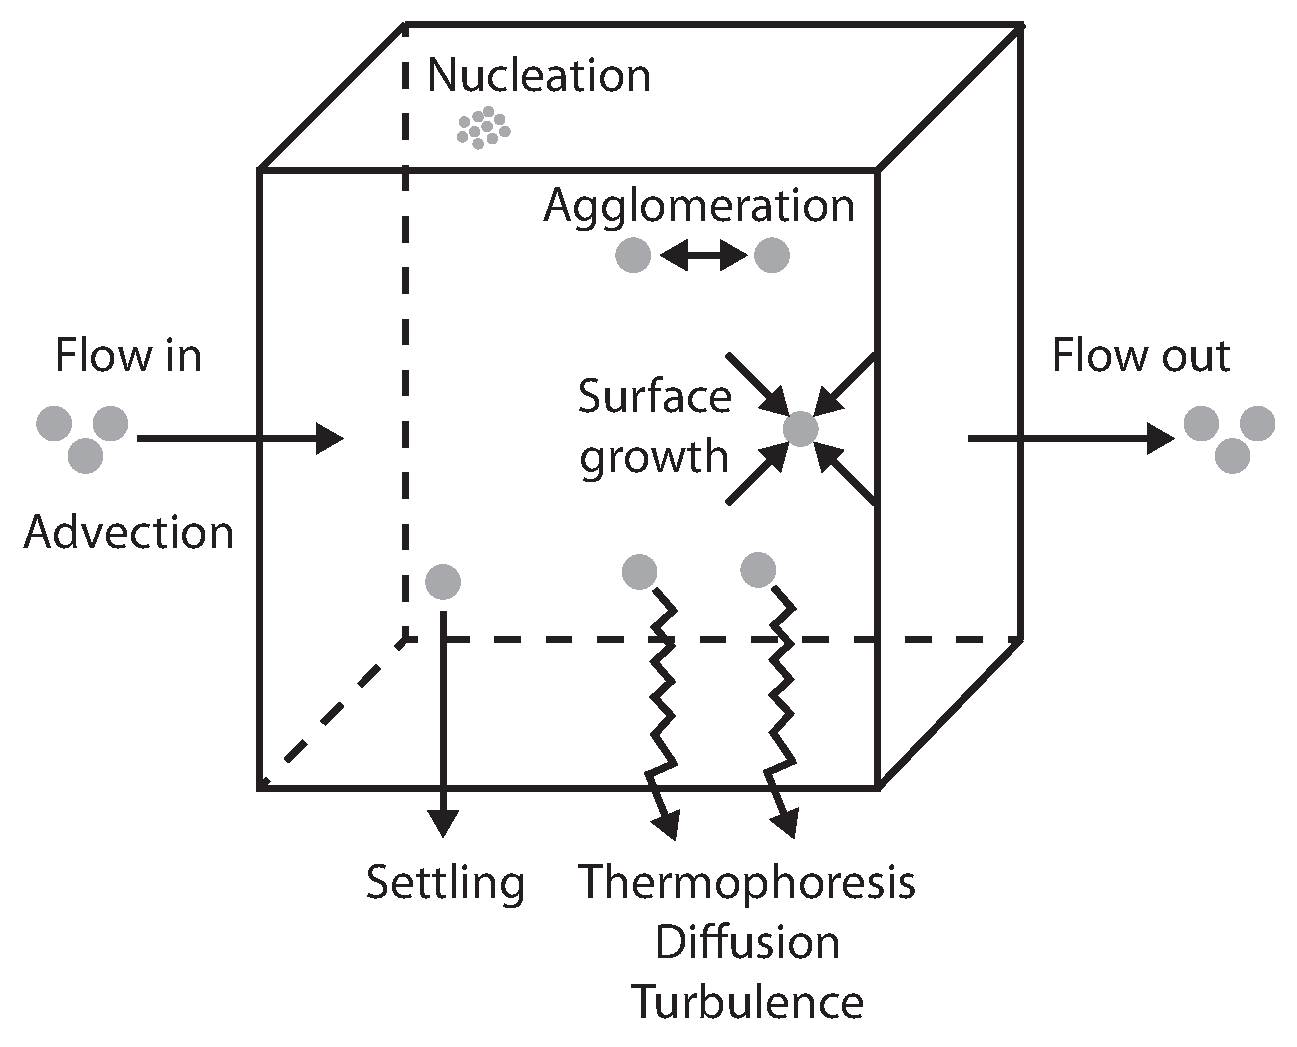
\includegraphics[width=5.0in]{Fig_Particle_Processes.pdf}
\caption[Soot transport, deposition, and agglomeration processes]{Soot transport, deposition, and agglomeration processes. Adapted from Friedlander~\cite{friedlander2000smoke}.}
\label{fig:particle_processes}
\end{figure}

Relatively simple parameterizations of soot chemistry and transport are incorporated into most computational fluid dynamics (CFD) fire models. Soot production is typically specified by means of a fixed soot yield for a given fuel. This assumption typically holds for well-ventilated fire scenarios in the open but has limitations in vitiated conditions and for potential advances in soot production modeling.

The underprediction of soot deposition on walls and surfaces in compartment fire scenarios can result in an overprediction of smoke concentrations in the gas phase~\cite{Butler:2004p433,Hamins:SP1013-1}. Soot deposition to walls can reduce the gas-phase soot concentration, which will tend to delay smoke detector activation and improve visibility. However, gravitational settling can result in increased obscuration in the lower layer. Gas-phase measurements of soot volume fraction used to parameterize soot generation models may be in error if significant deposition occurs. By not explicitly accounting for soot deposition on walls and surfaces, errors in soot concentration predictions in the gas phase can impact the calibration parameters for soot models. Errors in predicted quantities related to soot can affect life safety design decisions and can have adverse effects on performance goals related to both occupant safety and property protection~\cite{Cohan:Masters,riahi2013wall}. Soot deposition can also be used to reproduce fire and smoke patterns on surfaces, which can be beneficial in forensic fire reconstruction exercises.

Various aerosol/soot deposition mechanisms, including thermophoretic deposition (where temperature gradients push the aerosol towards or away from the surface), gravitational settling, molecular and turbulent diffusion (where the aerosols move along the boundary layer concentration gradient or deposit due to a turbulent boundary layer), and electrophoretic deposition can reduce the soot particle concentration in the gas phase by depositing soot on surfaces such as walls and ceilings. Soot agglomeration occurs at different scales and can increase the size of soot particles and affect soot deposition rates in both the flaming region and the post-flame environment~\cite{Butler:2004p433,mulholland1977coagulation}. As a first approach of quantifying aerosol deposition predictions under non-reacting flow conditions, this study identifies important parameters and physics related to aerosol deposition under various flow conditions. Aerosol deposition mechanisms will be compared, and predicted aerosol deposition rates will be compared to experimentally measured data. Because the experiments considered in this study were conducted under isothermal conditions, there is not an evaluation of the role of thermophoretic deposition in the total amount of deposited aerosol mass. Rather, this validation work focuses on the role of turbulent deposition and gravitational settling rather than thermophoretic deposition or soot agglomeration.

\section{Background}
\label{sec:Background}

Several studies have been conducted that indicate soot deposition is an important factor in compartment fires for the accurate prediction of smoke concentrations, smoke detector activations, and visibility. Gottuk et al.~\cite{Gottuk:IAFSS2008} reported that smoke concentrations predicted by Fire Dynamics Simulator (FDS) near smoke alarms in a corridor were two to five times greater than measured smoke concentrations. Hamins et al.~\cite{Hamins:SP1013-1} conducted full-scale compartment fire experiments for use in validation studies of various fire models, including FDS. The results indicated that smoke concentrations predicted by FDS were up to five times greater than measured smoke concentrations. Floyd and McDermott~\cite{Floyd:Interflam2010} implemented thermophoretic and turbulent diffusion soot deposition mechanisms in FDS and compared predicted soot concentrations to measurements from small- and large-scale experiments. Riahi~\cite{riahi2013wall} conducted bench-scale experiments to measure soot densities and soot deposition patterns on walls for various fuels. In those studies, Riahi identified thermophoretic deposition as an important soot deposition mechanism in a hot gas layer. Cohan~\cite{Cohan:Masters} used FDS to simulate select cases from the Gottuk~\cite{Gottuk:IAFSS2008} corridor tests, Hamins et al.~\cite{Hamins:SP1013-1} experiments, and Riahi~\cite{riahi2013wall} hood experiments with thermophoretic and turbulent diffusion soot deposition mechanisms. Newman et al.~\cite{newmansmoke} conducted experiments to quantify smoke deposition velocities and smoke damage to electrical components used in industrial facilities.

Soot formation and growth processes within a flame involve a range of different particle sizes. Initially, soot particles that form in a flame are on the order of a few nm~\cite{kennedy1997models}. As soot particles interact, collide, and stick to one another, they agglomerate to form larger particle sizes over time. Within the flame region, soot particle sizes can range between 0.02~$\mu$m and 0.05~$\mu$m~\cite{Butler:2004p433}, depending on the type of fuel. As the soot particles agglomerate in the post-flame environment, the particle size distribution can range from approximately 0.1~$\mu$m to 10~$\mu$m or larger, with peaks in the distribution that depend on the fuel, temperature, flow conditions, etc. Median aerodynamic diameters of soot particles can range from 0.05~$\mu$m for wood to 10~$\mu$m for acetylene, and a majority of fuels have median aerodynamic diameters less than 1~$\mu$m~\cite{Butler:2004p433}. High-sooting fuels, such as toluene and acetylene, can produce large soot particle sizes (or ``superaggregates'') ranging from 10~$\mu$m to 100~$\mu$m or larger~\cite{PhysRevLett.80.1782,doi:10.1021/la034063h,Kearney20123191}. In a CFD fire model such as FDS, grid cell sizes are typically on the order of 10~cm. At this coarse resolution, the flame sheet and dynamics of soot formation cannot be captured. In compartment fire scenarios, we are typically more interested in the bulk transport of soot and its effect on targets some distance from the fire. Therefore, this study focuses on implementing models and empirical correlations that describe soot transport and deposition using accurate, inexpensive techniques.

In soot transport algorithms, it is important to track a meaningful representation of the soot particle size because soot deposition and agglomeration mechanisms are dependent upon the size and stopping distance of the particles. The description and evolution of a detailed soot particle size distribution can be computationally expensive. A soot particle size distribution is shown in Fig.~\ref{fig:particle_size_distribution}. In this figure, $d\sb{p}$ is the particle size and $n(d\sb{p})$ is the number of particles in a given size bin. Rather than transporting detailed information about the particle size distribution (left side of Fig.~\ref{fig:particle_size_distribution}), the mean soot diameter $d\sb{p, mean}$ can be used to approximately describe and evolve the full soot particle size distribution (right side of Fig.~\ref{fig:particle_size_distribution}).

\begin{figure}[!ht]
\centering
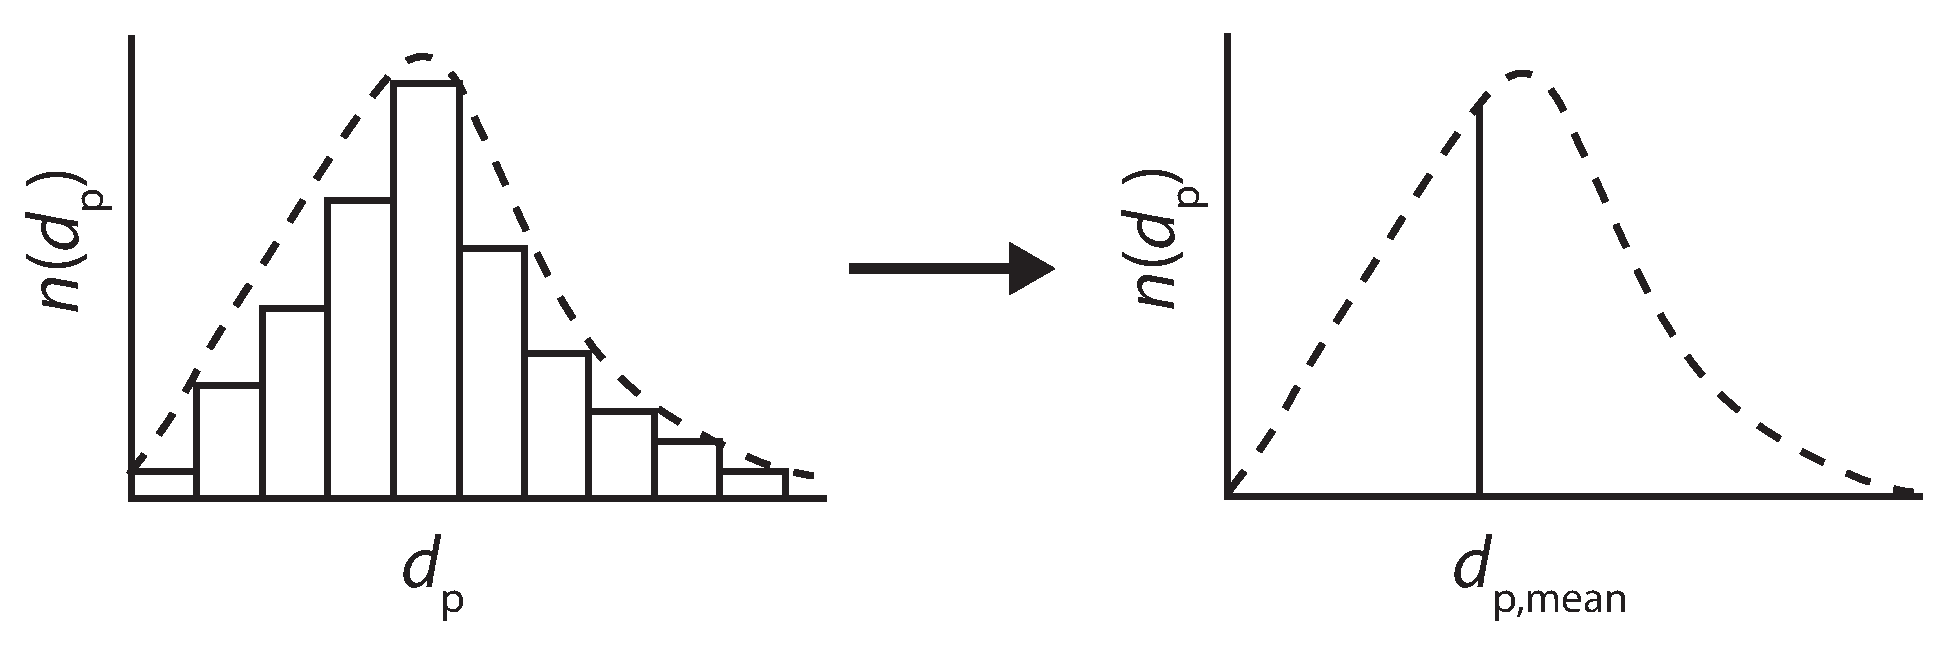
\includegraphics[width=5.0in]{Fig_Particle_Size_Distribution.pdf}
\caption[Detailed soot particle size distribution and mean particle size]
{Detailed particle size distribution (left) represented by mean particle size (right).}
\label{fig:particle_size_distribution}
\end{figure}

\section{Governing Equations}
\label{sec:Governing Equations}


\subsection{Soot Transport in Gas-Phase Cells}

If we define the mass fraction of an aerosol species $\alpha$ as $Y_\alpha = \rho_\alpha/\rho$, where $\rho_\alpha$ is the particle mass concentration and $\rho$ is the density of the gas~(kg/m$^3$), then the species transport equation is given by~\cite{FDS_Math_Guide}
\begin{equation}
\frac{\partial}{\partial t} (\rho Y_\alpha) + \nabla \cdot (\rho Y_\alpha \mathbf{u}) = \nabla \cdot (\rho D_\alpha \nabla Y_\alpha) + \dot m'''_\alpha
\label{eq:species_transport}
\end{equation}
where $Y_\alpha$ is the mass fraction of species $\alpha$~(kg/kg), $\mathbf{u}$ is the gas velocity~(m/s), $D_\alpha$ is the diffusivity of species $\alpha$~(m$^2$/s), and $\dot m'''_\alpha$ is the source term for species $\alpha$ (kg/m$^3$-s), which can be specified via a bulk mass production rate or a chemical mass production or consumption rate.

For each aerosol species in the gas phase, a gravitational settling velocity is calculated and imposed on the velocity in the convective term in the species transport equation, which results in the following modified form of the equation for aerosols
\begin{equation}
\frac{\partial}{\partial t} (\rho Y_\alpha) + \nabla \cdot (\rho Y_\alpha \mathbf{U}) = \nabla \cdot (\rho D_\alpha \nabla Y_\alpha) + \dot m'''_\alpha
\label{eq:modified_species_transport}
\end{equation}
where $\mathbf{U}$ is the relative particle velocity~(m/s), which can be decomposed into the gas velocity and particle velocity as $\mathbf{u + u\sb{p}}$.

In the modified form of the species transport equation (Eq.~\ref{eq:modified_species_transport}), the particle velocity $\mathbf{u\sb{p}}$ is equal to the gravitational settling velocity $\mathbf{u\sb{g}}$. This approach is similar to the drift flux model for smoke transport described in Hu et al.~\cite{Hu:1}. In Eq.~\ref{eq:modified_species_transport}, soot deposition is imposed as a boundary flux condition at surfaces, which is described in the following section.

\subsection{Soot Deposition to Surfaces}

Adapting Eq.~\ref{eq:modified_species_transport} for one dimensional flux towards a surface, the change in the soot mass fraction ($\rho Y_{\alpha}$) in a control volume results in a boundary condition for which soot is removed from the gas-phase and deposited onto the wall surface at the rate $\dot m''$, which is given by
\begin{equation}
\dot m'' = \rho Y_\alpha u\sb{dep}
\label{eq:soot_deposition_bc}
\end{equation}
Using this flux condition, the amount of aerosol that deposits on the surface is removed from the adjacent gas-phase cell, and the amount of aerosol that accumulates on the surface is tracked.

The total aerosol deposition velocity to surfaces, $u\sb{dep}$, is determined by assuming the deposition phenomena are independent, computing a deposition velocity for each mechanism, and then summing
them as~\cite{Bixler:1}
\begin{equation}
u\sb{dep} = u\sb{g}+u\sb{th}+u\sb{dt}
\label{eq:total_soot_deposition}
\end{equation}
where $u\sb{g}$ is the gravitational settling velocity (for gas-phase cells adjacent to upward-facing surfaces), $u\sb{th}$ is the thermophoretic velocity, and $u\sb{dt}$ is the combined diffusion-turbulence velocity. These deposition mechanisms will be discussed in more detail in the following sections.

\subsection{Gravitational Settling}
\label{sec:gravitational_settling}

Gravitational deposition occurs due to the force of gravity acting on particles, which results in a downward gravitational settling velocity. As the size of a particle increases, the gravitational force on the particle also increases. The gravitational settling velocity is given by~\cite{Davies_Charles}
\begin{equation}
u\sb{g} = g m\sb{a} \frac{\textrm{Cn}}{6 \pi \, \chi\sb{d} \, \mu \, r\sb{a}}
\end{equation}
where $m\sb{a}$ is the particle mass and is constant, $\chi\sb{d}$ is the shape factor, $\mu$ is the dynamic viscosity of air, $r\sb{a}$ is the particle radius and is constant, and Cn is the Cunningham slip correction factor given by~\cite{Cunningham:1}
\begin{equation}
\textrm{Cn} = 1 + 1.25 \; \textrm{Kn} + 0.41 \; \textrm{Kn} \; \mathrm{e}^{-0.88/\textrm{Kn}}
\label{eq:Cn}
\end{equation}
where Kn is the particle Knudsen number given by the ratio of the mean free path of the gas to the particle radius. The mean free path of a gas is proportional to its temperature, thus Kn is computed as~\cite{Sippola:1}
\begin{equation}
\textrm{Kn} = \frac{\lambda}{r\sb{a}} \frac{T\sb{g}}{T_\infty}
\end{equation}
where $\lambda$ is the mean free path of gas molecules and is equal to~0.065~$\mu$m at a temperature of 25~$^\circ$C and atmospheric pressure.

\subsection{Thermophoretic Deposition}
\label{sec:thermophoretic_deposition}

Thermophoretic deposition is the result of a temperature gradient near a surface, which can attract particles towards or repel particles away from a nearby surface. The thermophoretic velocity is computed as
\begin{equation}
u\sb{th} = \frac{K\sb{th} \nu}{T\sb{g}} \; \frac{dT}{dx}
\label{eq:thermophoretic}
\end{equation}
where $\nu$ is the kinematic viscosity of air, and $T\sb{g}$ is the gas temperature. This requires the calculation of the wall temperature gradient $dT/dx$, which is only resolved in a direct numerical simulation (DNS) with very small grid cell sizes. For a large eddy simulation (LES) with larger grid cell sizes, the temperature gradient is computed from the wall heat transfer coefficient $h$ as
\begin{equation}
 \frac{dT}{dx} = \frac{h \left( T\sb{g} - T\sb{w} \right)}{k\sb{g}}
\end{equation}
where $T\sb{w}$ is the wall temperature, and $k\sb{g}$ is the thermal conductivity of air. In Eq.~\ref{eq:thermophoretic}, $K\sb{th}$ is the thermophoretic velocity coefficient and is calculated using the following correlation~\cite{Brock:1}
\begin{equation}
 K\sb{th} = \frac{2 \, C\sb{s} \left(\alpha + C\sb{t} \; \textrm{Kn} \right) \; \textrm{Cn}}{\left(1 + 3 \, C\sb{m} \; \textrm{Kn} \right) \left(1 + 2 \, \alpha + 2 \, C\sb{t} \, \textrm{Kn} \right) }
\end{equation}
where $C\sb{s}=1.17$ is the thermal slip coefficient, $\alpha$ is the ratio of the gas conductivity to the particle conductivity~($k\sb{g}/k\sb{solid}$), $C\sb{m}=1.14$ is the momentum accommodation coefficient, and $C\sb{t}=2.18$ is the thermal accommodation coefficient.

\subsection{Turbulent Deposition}
\label{sec:turbulent_deposition}

In turbulent flow conditions near surfaces, turbulent deposition can occur when the inertia of particles within the flow causes them to separate from the flow, impact a surface, and deposit (or stick) to the surface.

The diffusion-turbulence deposition velocity depends upon the flow regime (diffusion, diffusion-impaction, or inertia-moderated). The deposition velocity for these regimes is given as~\cite{McCoy_Hanratty}
\begin{equation}
u\sb{dt} = \left\{ \begin{array}{r@{\quad \quad}l}
         0.086 \; \textrm{Sc}^{-0.7} \; u_{\tau}        &  \tau^+ < 0.2 \\
         3.5 \times 10^{-4} \; {\tau^+}^2 \; u_{\tau} &  0.2 < \tau^+ < 22.9 \\
         0.17 \; u_{\tau}                             &  \tau^+ < 22.9
         \end{array} \right.
\end{equation}
where Sc is the particle Schmidt number, or the ratio of the kinematic viscosity of air to the Brownian diffusion coefficient of the particle ($\nu/D\sb{B}$), $u_{\tau}$~is the wall friction velocity computed by the wall model, or $\sqrt{\tau\sb{w}/\rho}$~(where $\tau\sb{w}$ is the wall shear stress and $\rho$ is the density of air), and $\tau^+$ is the dimensionless stopping distance of the particle given by~\cite{Ludwig_ICONE}
\begin{equation}
 \tau^+=\frac{\rho\sb{a} \, (2 r\sb{a})^2}{18 \, \mu^2}  \; u_{\tau}^2 \; \rho\sb{g}
\end{equation}
The Brownian diffusion coefficient~$D\sb{B}$ of a particle is given by
\begin{equation}
D\sb{B} = \frac{k T \sb{Cn}}{3 \pi \mu d}
\end{equation}
where $k$ is the Boltzmann constant~($1.38 \times 10^{-23}$~J/K), $T$ is the gas temperature, Cn is the Cunningham slip factor given in Eq.~\ref{eq:Cn}, $\mu$ is the dynamic viscosity of air, and $d$ is the particle diameter and is constant.

\subsection{Numerical Implementation}

In summary, the velocity in the convective term in Eq.~\ref{eq:species_transport} for a tracked aerosol species was modified in FDS version 6.0.0 to include the gravitational settling velocity $u\sb{g}$. For soot deposition to surfaces, the FDS source code for gas-phase cells adjacent to walls was modified to include gravitational, thermophoretic, and turbulent deposition mechanisms as a boundary flux condition using Eqs.~\ref{eq:soot_deposition_bc} and~\ref{eq:total_soot_deposition}. A schematic of soot transport in FDS for various deposition mechanisms in a compartment is shown in Fig.~\ref{fig:soot_deposition_schematic}. For computational cells near the ceiling or wall, the aerosol deposition velocity includes thermophoretic and turbulent mechanisms. For computational cells near the floor, the aerosol deposition velocity includes gravitational, thermophoretic, and turbulent mechanisms. For computational cells that are not near surfaces, the aerosol velocity includes the gas velocity and the gravitational settling velocity. These modifications allow for the removal of soot from the gas phase and the accumulation of soot on surfaces due to the deposition and settling of aerosols.

\begin{figure}[!ht]
\centering
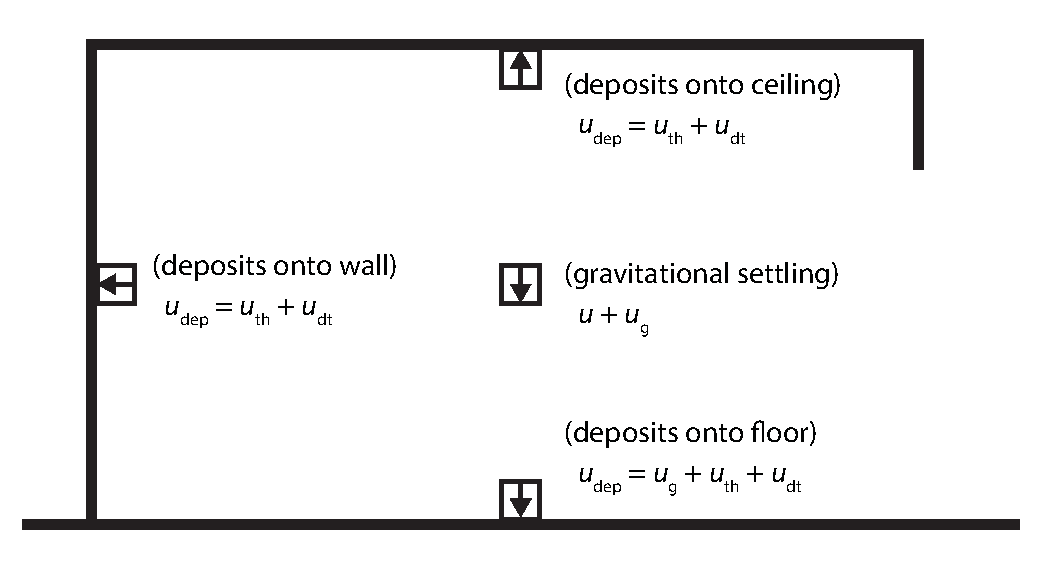
\includegraphics[width=5.0in]{Fig_Soot_Deposition_Schematic.pdf}
\caption[Soot deposition in FDS via various mechanisms]{Soot deposition in a simplified compartment via various mechanisms. Representative computational cells are shown in four different locations: one in the middle of the compartment, and three others near the ceiling, wall, and floor.}
\label{fig:soot_deposition_schematic}
\end{figure}

\section{Experimental Setup}
\label{sec:Experimental Setup}

To assess the accuracy of the aerosol deposition model under simplified (non-fire) conditions, model predictions will be compared to experiments conducted in a nonreacting flow system. Experimental data measured by Sippola~\cite{Sippola:2002,Sippola:2010} were identified as a suitable candidate for model validation because the tests had well-characterized geometry and flow conditions, monodisperse aerosol sizes, and separate measurements of the ceiling, wall, and floor deposition velocities.

Sippola measured aerosol deposition velocities for various sizes of monodisperse fluorescent particles and various air velocities in a ventilation duct~\cite{Sippola:2002,Sippola:2010}. For the experiments considered here, a total of 16 aerosol deposition tests were conducted in a steel duct system. The duct had smooth walls and was square with cross-sectional dimensions of 15~cm by 15~cm. The particle diameters were 1~$\mu$m, 3~$\mu$m, 5~$\mu$m, 9~$\mu$m, and 16~$\mu$m, which is within the range of soot particle sizes that would be expected in a fire scenario~(see Section~\ref{sec:Background}). The air velocities in the duct were 2.2~m/s, 5.3~m/s, and 9.0~m/s with Reynolds numbers of approximately 22,000; 53,000; and 89,000, respectively. The air velocity in the duct was verified by using the average value of 16 air velocity measurements via pitot tubes arranged in a 4 by 4 grid immediately upstream of the aerosol deposition test panels.

Twelve panels measuring 20~cm by 10~cm were cut from an instrumented duct section and used to measure the amount of particles deposited on the duct surfaces: four panels each from the duct ceiling, wall, and floor surfaces. Fluorescent measurement techniques and aerosol concentration measurements were used to calculate the deposition velocities of the particles to duct surfaces (ceiling, wall, and floor) at a straight duct section where the turbulent flow profile was fully developed. Sippola reported a 10~\% relative experimental uncertainty in the measured aerosol deposition velocities~\cite{Sippola:2002}. 

Figure~\ref{fig:Sippola_Diagram_1} shows a schematic of the experimental setup. Figure~\ref{fig:Sippola_Diagram_2} shows a detailed view of Section~2 in the duct and the panels that were used to collect the deposited aerosol and calculate the aerosol deposition velocity. A summary of the 16 aerosol deposition tests is shown in Table~\ref{tab:Sippola_Aerosol_Deposition_Summary}.

\begin{figure}[!ht]
\centering
\subfloat[Overview of experimental setup. The shaded region was modeled in FDS.]{\label{fig:Sippola_Diagram_1}
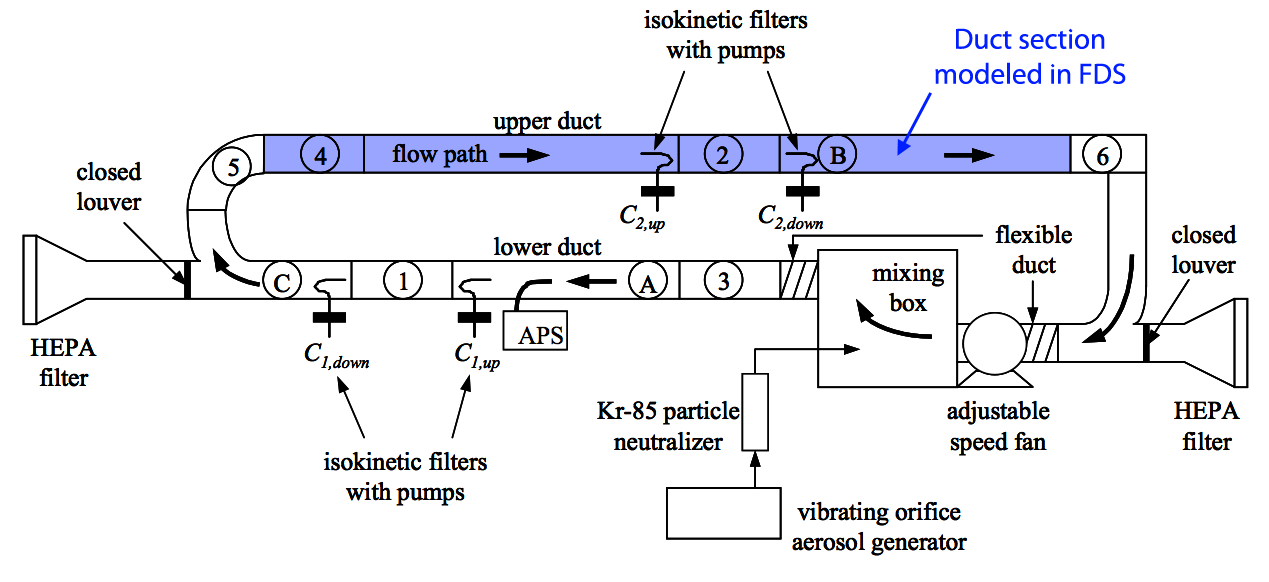
\includegraphics[width=5.0in]{Fig_Sippola_Diagram.png}}
\qquad
\subfloat[Detailed view of instrumented duct Section~2]{\label{fig:Sippola_Diagram_2}
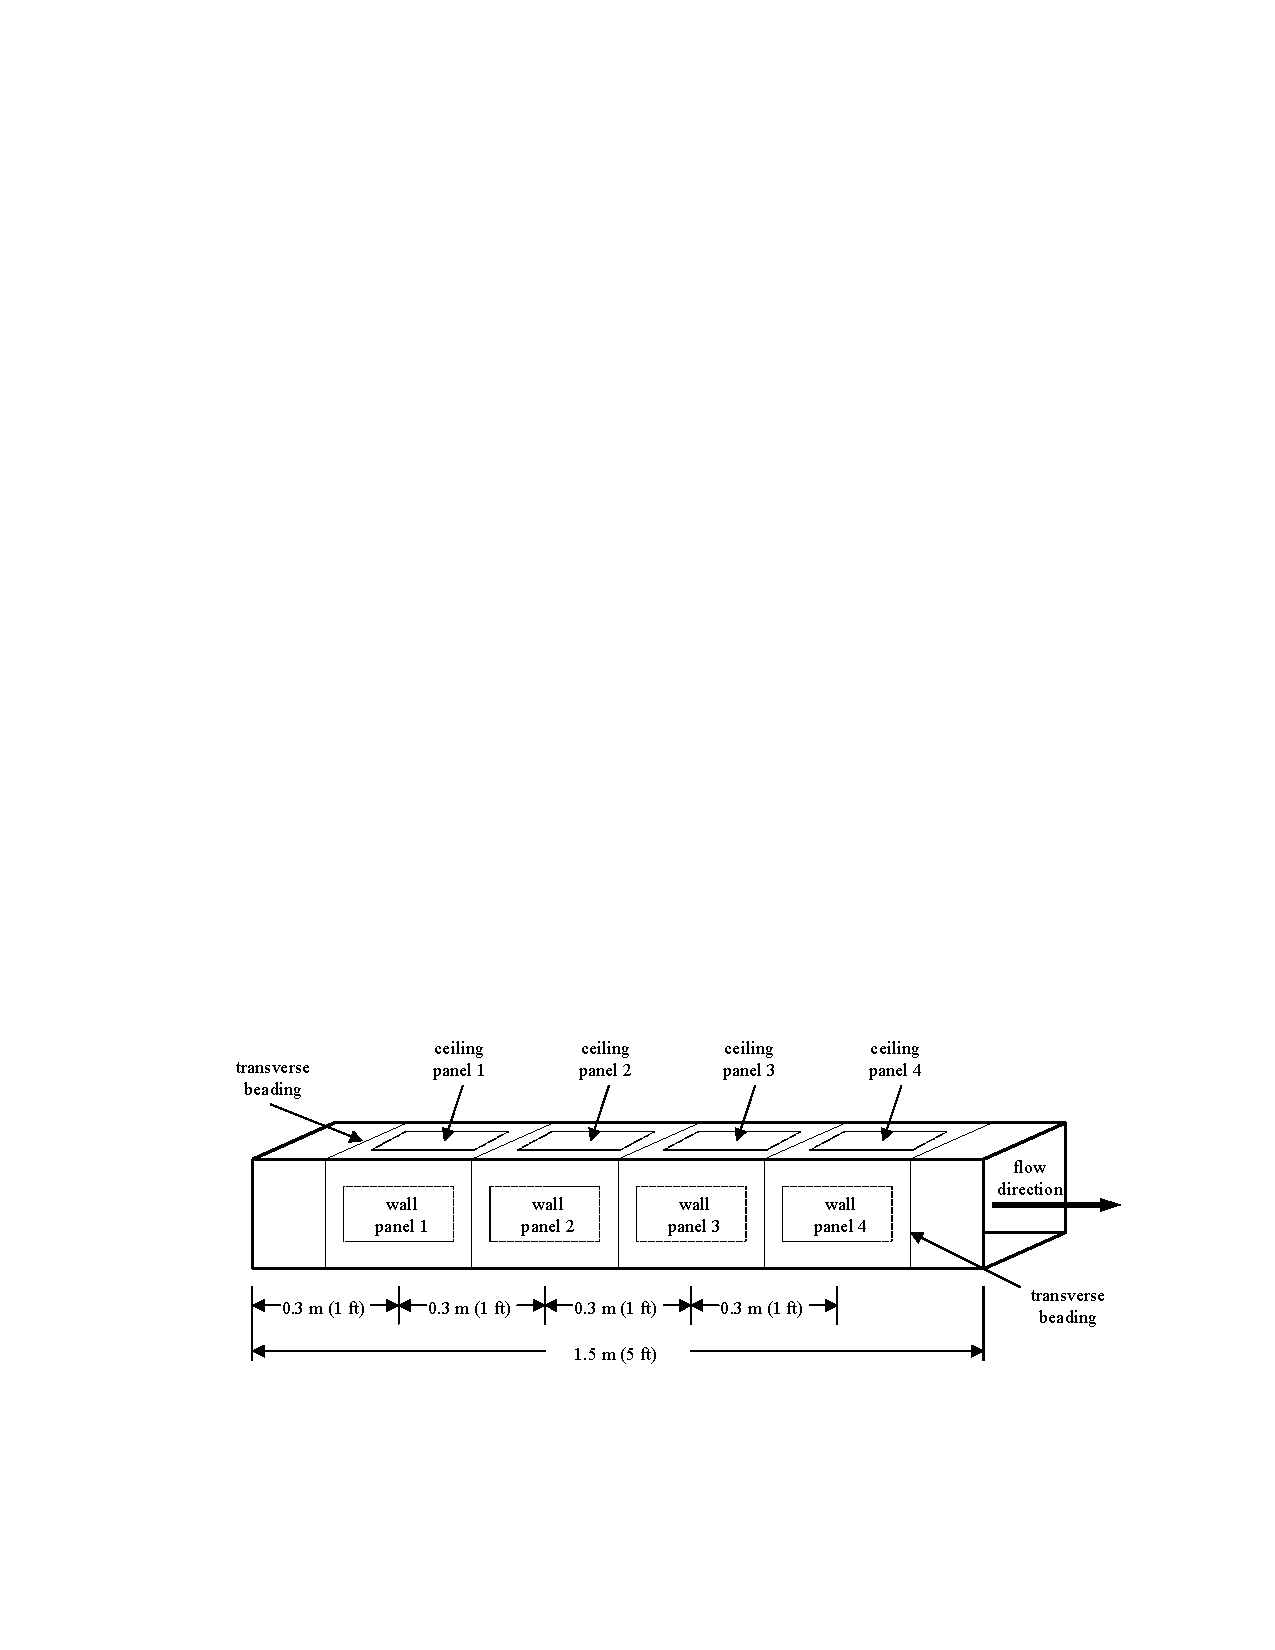
\includegraphics[width=5.0in]{Fig_Sippola_Aerosol_Deposition_Duct_Detail.pdf}}
\caption[Experimental setup used in Sippola aerosol deposition experiments]
{Schematic of experimental apparatus used in Sippola aerosol deposition experiments~\cite{Sippola:2002}.}
\label{fig:Sippola_Diagram}
\end{figure}

\begin{table}[!ht]
\centering
\caption[Summary of Sippola aerosol deposition experiments]
{Summary of Sippola aerosol deposition experiments performed in a duct.}
\begin{tabular}{ccccc}
\hline\noalign{\smallskip}
Test      &  Air     &  Particle  &  Particle    &  Ambient      \\
Number    &  Speed   &  Diameter  &  Density     &  Temperature  \\
          &  (m/s)   &  ($\mu$m)  &  (kg/m$^3$)  &  ($^\circ$C)  \\
\noalign{\smallskip}\hline\noalign{\smallskip}
1         &  2.2     &  1.0       &  1350        &  22.0         \\
2         &  2.2     &  2.8       &  1170        &  22.0         \\
3         &  2.1     &  5.2       &  1210        &  21.8         \\
4         &  2.2     &  9.1       &  1030        &  22.2         \\
5         &  2.2     &  16        &  950         &  22.4         \\
6         &  5.3     &  1.0       &  1350        &  24.1         \\
7         &  5.2     &  1.0       &  1350        &  23.0         \\
8         &  5.2     &  3.1       &  1170        &  23.0         \\
9         &  5.4     &  5.2       &  1210        &  22.9         \\
10        &  5.3     &  9.8       &  1030        &  23.0         \\
11        &  5.3     &  16        &  950         &  23.1         \\
12        &  9.0     &  1.0       &  1350        &  26.9         \\
13        &  9.0     &  3.1       &  1170        &  25.4         \\
14        &  8.8     &  5.4       &  1210        &  25.6         \\
15        &  9.2     &  8.7       &  1030        &  25.9         \\
16        &  9.1     &  15        &  950         &  25.9         \\
\noalign{\smallskip}\hline
\end{tabular}
\label{tab:Sippola_Aerosol_Deposition_Summary}
\end{table}


\clearpage


\section{Computational Setup}
\label{sec:Computational Setup}

Figure~\ref{fig:Sippola_Diagram_1} shows a schematic of the experimental setup and the 5~m duct section that was modeled (blue shaded section). In the model, an additional 3~m of duct section (equal to 20~duct diameters) was included upstream of the instrumented portion of the duct (Section~2) to allow for the flow to become fully developed.

In the numerical simulations, the grid cell size was 1~cm on all sides. The air velocity in the duct was specified for each test as an upstream inlet boundary condition, and the outlet was specified as an open boundary condition (open to ambient conditions). The duct walls were specified as a 1-mm thick, smooth material. The wall thickness did not impact the aerosol deposition rate, but is a required input parameter and is included for completeness and reproducibility. All of the experiments were isothermal, and thus this validation will focus on the accuracy of the aerosol deposition results with respect to the gravitational settling and turbulent deposition mechanisms.

In the simulations, the aerosol species was tracked explicitly, and all of the aerosol deposition mechanisms were enabled. The measured aerosol concentrations were not given in the test reports; therefore, an aerosol concentration of 100~mg/m$^3$ was specified at the inlet (upstream) duct boundary.

\section{Results}
\label{sec:Results}

\subsection{Aerosol Deposition Velocity}

In the experimental setup, there was only one upstream and one downstream concentration measurement available. Therefore, to make an accurate comparison between the measured and predicted deposition velocities, we will use the same data reduction technique as Sippola~\cite{Sippola:2002,Sippola:2010}.

Following the procedure by Sippola, the particle deposition velocity $V\sb{d}$ was calculated as
\begin{equation}
V\sb{d} = \frac{J\sb{1} + J\sb{2} + J\sb{3} + J\sb{4}}{4 \; C\sb{avg}}
\label{eq:sippola_deposition_velocity}
\end{equation}
where~$J\sb{1}$ through~$J\sb{4}$ are the deposition fluxes (kg/m$^2$-s) for duct panels~1 through~4, respectively, which is given by
\begin{equation}
J = \frac{\Delta m\sb{d}}{A\sb{d} \; \Delta t}
\label{eq:sippola_deposition_flux}
\end{equation}
where $\Delta m\sb{d}$ is the change in mass on the duct panel (kg), $A\sb{d}$ is the area of the duct panel (m$^2$), $\Delta t$ is the duration over which the aerosol deposits on the panel~(s), and $C\sb{avg}$ is the average of the upstream and downstream aerosol concentration in the duct test section (kg/m$^3$).

Figures~\ref{fig:Sippola_Aerosol_Deposition_Velocity_1} through~\ref{fig:Sippola_Aerosol_Deposition_Velocity_3} show comparisons of the measured and predicted aerosol deposition velocities for the ceiling, wall, and floor surfaces. Figure~\ref{fig:Summary_Aerosol_Deposition_Velocity} shows a summary of the measured and predicted results for all of the particle sizes, duct velocities, and surfaces that were considered. The model generally underpredicts the measured aerosol deposition velocity by 45~\%, on average.

\begin{figure}[p]
\centering
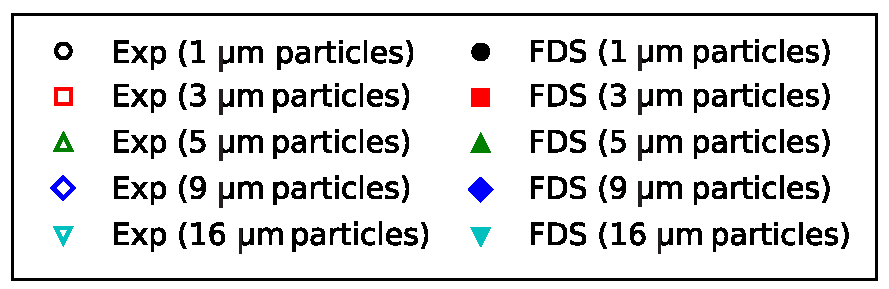
\includegraphics[width=3.8in]{Fig_Sippola_Aerosol_Deposition_Legend.pdf} \\
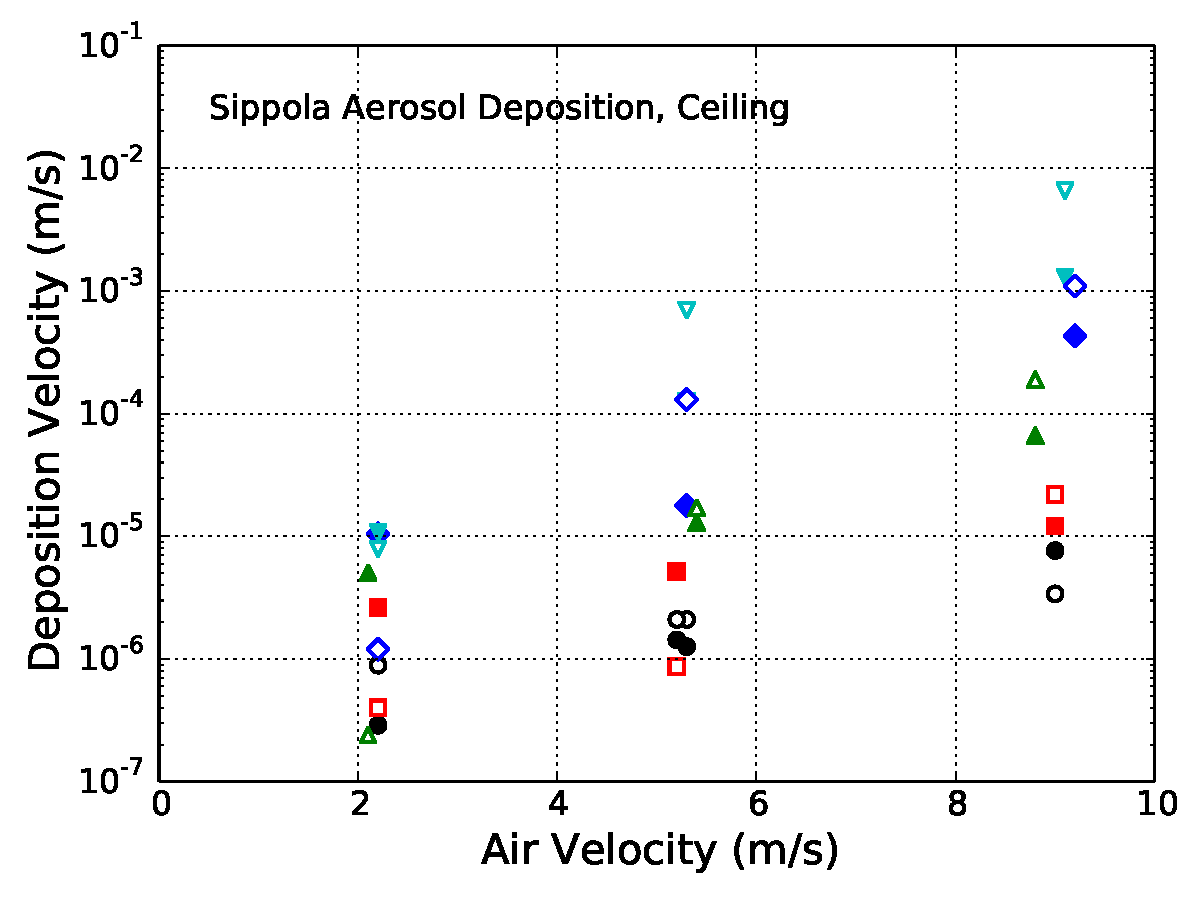
\includegraphics[width=5.0in]{Fig_Sippola_Aerosol_Ceiling_Deposition.pdf}
\caption[Ceiling aerosol deposition velocities]
{Measured and predicted ceiling aerosol deposition velocities.}
\label{fig:Sippola_Aerosol_Deposition_Velocity_1}
\end{figure}

\begin{figure}[p]
\centering
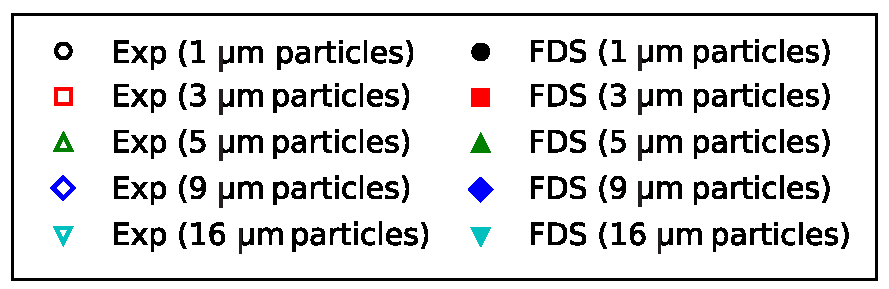
\includegraphics[width=3.8in]{Fig_Sippola_Aerosol_Deposition_Legend.pdf} \\
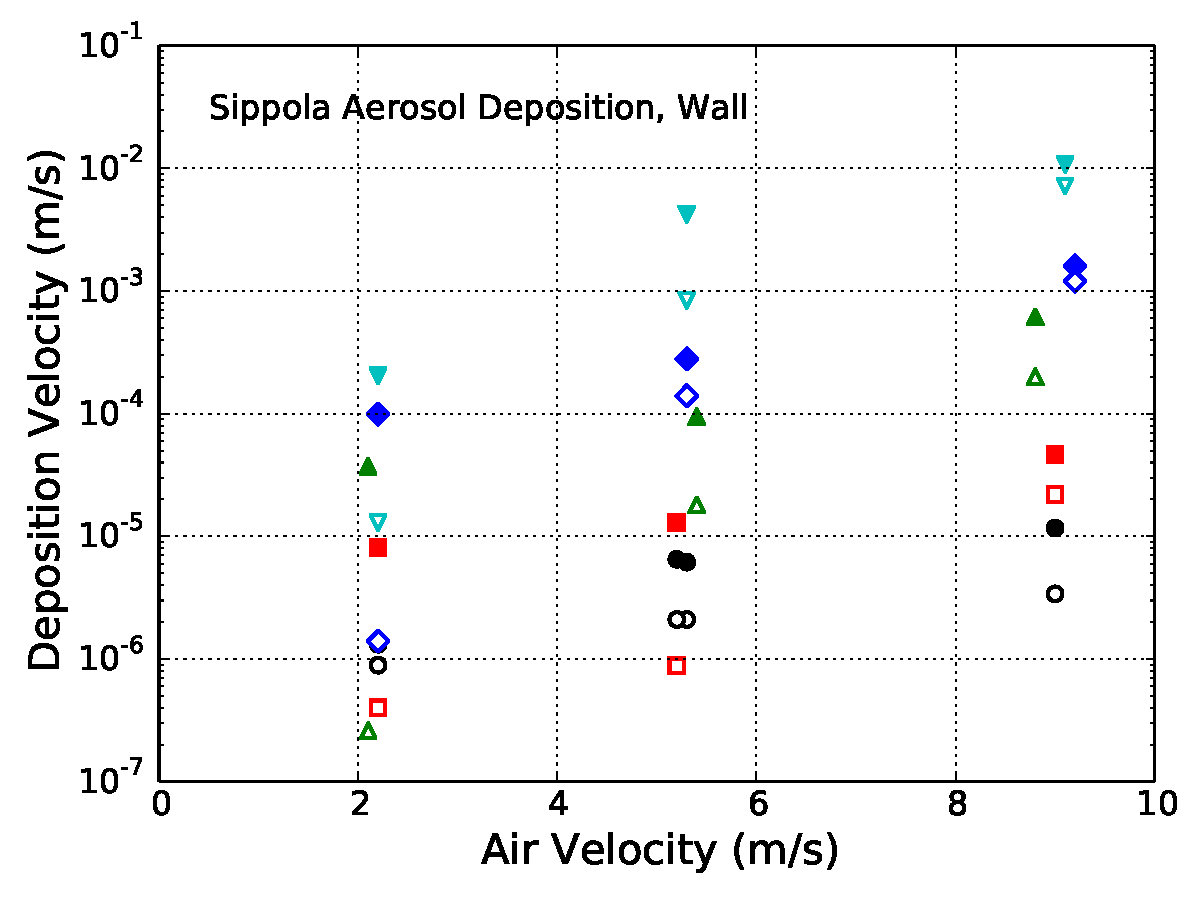
\includegraphics[width=5.0in]{Fig_Sippola_Aerosol_Wall_Deposition.pdf}
\caption[Wall aerosol deposition velocities]
{Measured and predicted wall aerosol deposition velocities.}
\label{fig:Sippola_Aerosol_Deposition_Velocity_2}
\end{figure}

\begin{figure}[p]
\centering
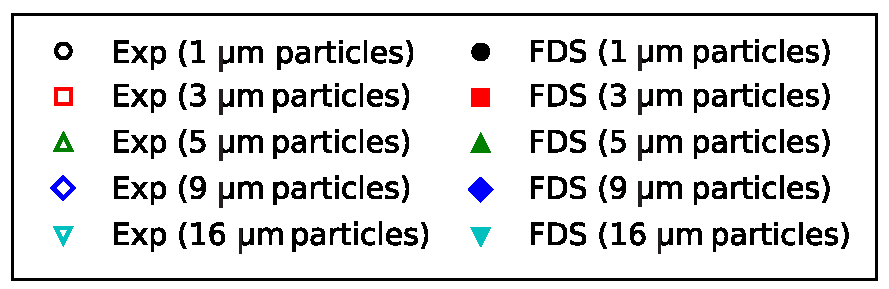
\includegraphics[width=3.8in]{Fig_Sippola_Aerosol_Deposition_Legend.pdf} \\
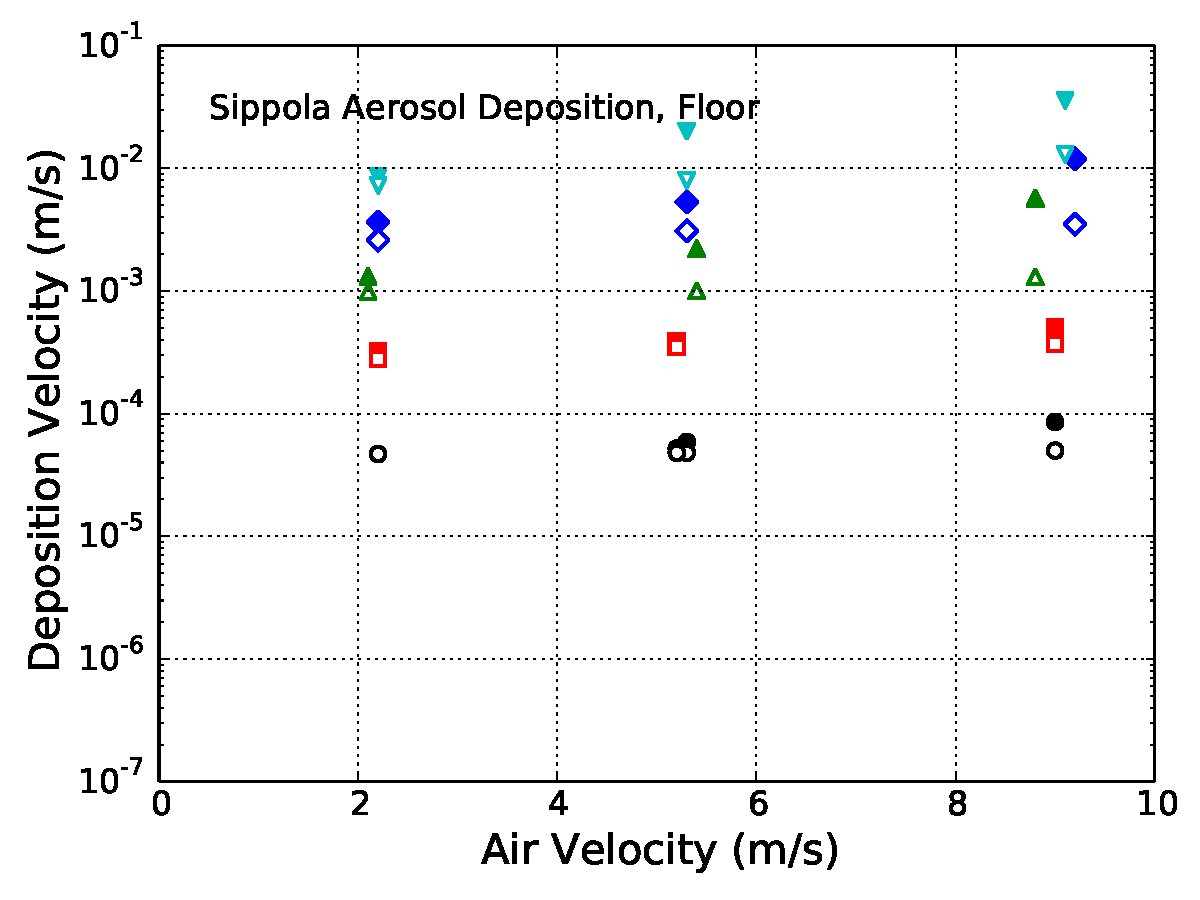
\includegraphics[width=5.0in]{Fig_Sippola_Aerosol_Floor_Deposition.pdf}
\caption[Floor aerosol deposition velocities]
{Measured and predicted floor aerosol deposition velocities.}
\label{fig:Sippola_Aerosol_Deposition_Velocity_3}
\end{figure}

\begin{figure}[!ht]
\centering
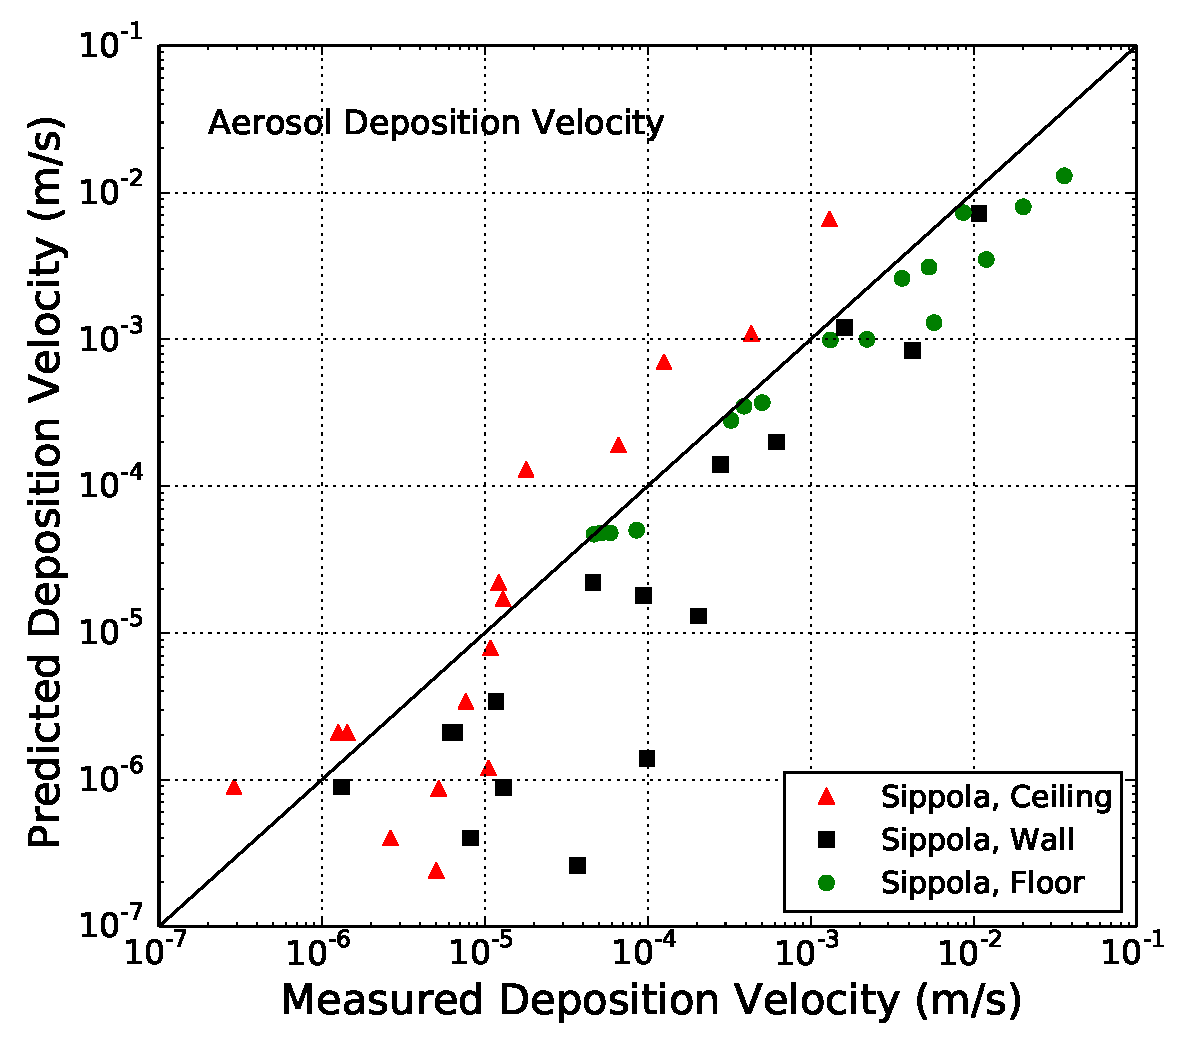
\includegraphics[width=5.0in]{Fig_Sippola_Aerosol_Deposition_Velocity_Scatter.pdf} \\
\caption[Summary of aerosol deposition velocities]
{Summary of aerosol deposition velocities.}
\label{fig:Summary_Aerosol_Deposition_Velocity}
\end{figure}

For all of the cases that were considered, the results indicate that, as the duct velocity and particle size increase, the deposition velocity also increases. The ceiling and wall aerosol deposition velocities ranged from approximately $1 \times 10^{-7}$~m/s to $1 \times 10^{-2}$~m/s. The floor aerosol deposition velocities ranged from approximately $1 \times 10^{-5}$~m/s to $1 \times 10^{-1}$~m/s, which is most likely due to the effect of gravitational settling.

For the model predictions, the effect of increased particle sizes was the greatest for the floor aerosol deposition velocities, and the effect of increased duct velocity was the greatest for the wall and ceiling. The floor aerosol deposition velocities were the least sensitive to an increase in the duct velocity because gravitational settling was more dominant than turbulent deposition at the floor.

The cases that exhibited the largest error in the predicted aerosol deposition velocities were the 3~$\mu$m and 5~$\mu$m particle sizes at the lowest air velocities, especially at the wall. The measured deposition velocity for these cases is on the order of $1 \times 10^{-5}$~m/s, which is a relatively small deposition velocity and would result in only a small amount of error in the deposited aerosol mass, as demonstrated in the following example.

Consider the case with the lowest air velocity (2.2~m/s). For an aerosol concentration of 100~mg/m$^3$ and a time period of 100~s, a total of 495~mg of aerosol mass flows through the duct. Using Eqs.~\ref{eq:sippola_deposition_velocity} and~\ref{eq:sippola_deposition_flux} with an aerosol deposition velocity of $1 \times 10^{-5}$~m/s and representative values from the Sippola experiments (aerosol concentration of 100~mg/m$^3$, deposition area of 0.02~m$^2$, and time of 100~s) results in only 0.002~mg of deposited aerosol mass out of the 495~mg of total aerosol mass that flowed through the duct. Therefore, errors in the relatively small deposition velocities (on the order of $1 \times 10^{-5}$~m/s) would not result in a significant amount of error in the deposited aerosol mass.

The remaining cases that used other particle sizes and duct velocities represent our best current ability to predict aerosol deposition velocities for the Sippola Aerosol Deposition experiments using FDS. In the following section, we will explore predicted quantities that were not measured in the experiments to understand some of the more detailed aerosol physics that might affect deposition rates.

\subsection{Velocity and Aerosol Concentration Gradients}

Figure~\ref{fig:Sippola_Aerosol_Deposition_Concentration} shows the predicted aerosol concentration along the centerline of the duct where the measurements were made. The results indicate that the aerosol concentration for the 1~$\mu$m particles remains nearly constant at approximately 98~mg/m$^3$. The aerosol concentration for the 16~$\mu$m particles at the highest air velocity decreases from approximately 92~mg/m$^3$ to 78~mg/m$^3$ because the larger particle size and higher air velocity result in a higher aerosol deposition velocity.

\begin{figure}[!ht]
\centering
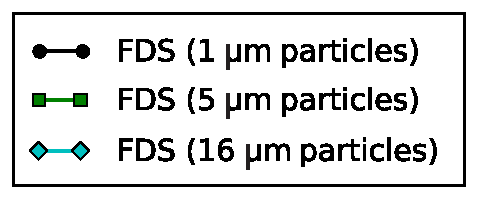
\includegraphics[width=2.4in]{Fig_Sippola_Aerosol_Deposition_Legend_Lines.pdf} \\
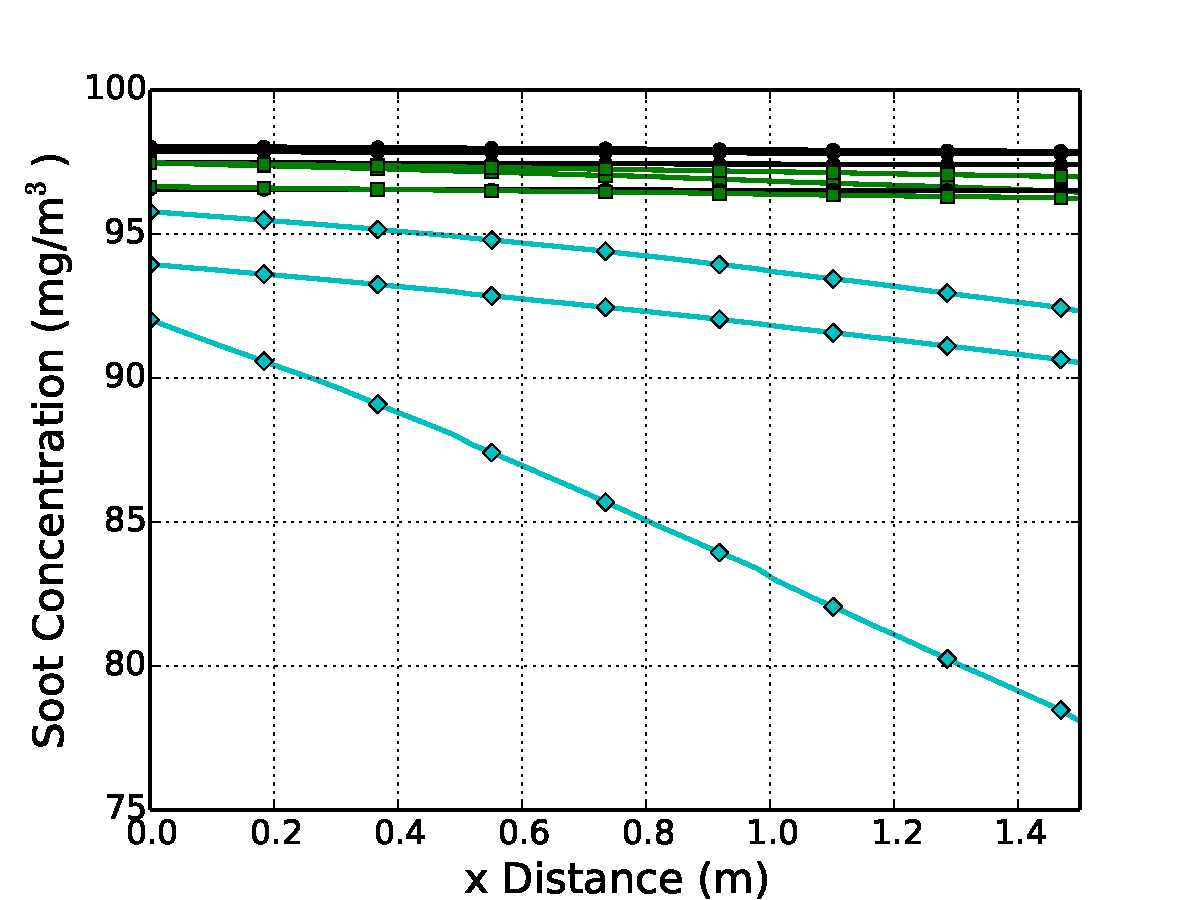
\includegraphics[width=5.0in]{Fig_Sippola_Aerosol_Deposition_Soot_Concentration_All.pdf}
\caption[Predicted aerosol concentration, Sippola Aerosol Deposition]
{Predicted aerosol concentration along the duct, Sippola Aerosol Deposition.}
\label{fig:Sippola_Aerosol_Deposition_Concentration}
\end{figure}

\noindent Figure~\ref{fig:Sippola_Transverse_Velocity} shows the predicted vertical air velocity profile in the duct for Tests~1 and 16 at a downstream location of 0.75~m, which is the midpoint in the 1.5~m instrumented section of the duct.

\begin{figure}[!ht]
\centering
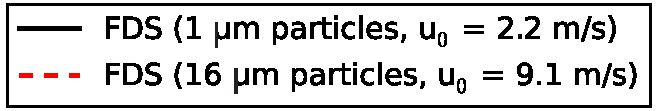
\includegraphics[width=3.5in]{Fig_Sippola_Aerosol_Deposition_Transverse_Legend.pdf}
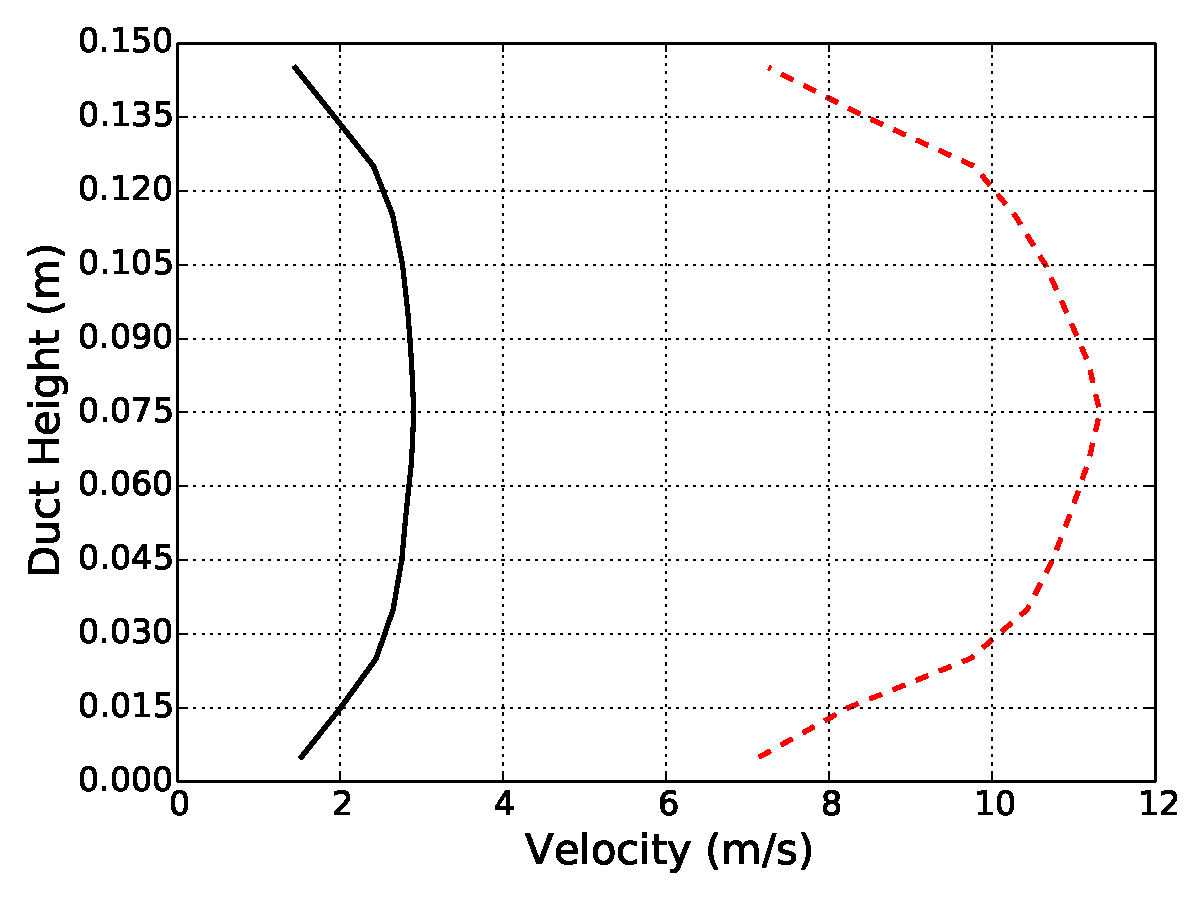
\includegraphics[width=5.0in]{Fig_Sippola_Aerosol_Deposition_Transverse_Velocity.pdf}
\caption[Vertical air velocity profile, Sippola Aerosol Deposition]
{Vertical air velocity profile 0.75~m downstream in the 1.5~m instrumented section of the duct for Test~1, 2.2~m/s case (solid line) and Test~16, 9.1~m/s case (dashed line), Sippola Aerosol Deposition.}
\label{fig:Sippola_Transverse_Velocity}
\end{figure}

The velocity in Test~1 was approximately 3.0~m/s near the duct centerline and 1.5~m/s near the duct walls. The velocity in Test~16 was approximately 11.8~m/s near the duct centerline and 6.8~m/s near the duct walls.

\noindent Figure~\ref{fig:Sippola_Transverse_Concentration} shows the predicted vertical aerosol concentration profile in the duct for Tests~1 and 16 at a downstream location of 0.75~m in the 1.5~m instrumented duct section. In this figure, it is evident that there is a change in aerosol concentration along the length of the duct section that was considered. This change in concentration is more prominent for larger particle sizes. The aerosol concentration in Test~1 was approximately 98~mg/m$^3$ near the duct ceiling and 99~mg/m$^3$ near the duct floor. The aerosol concentration in Test~16 was approximately 56~mg/m$^3$ near the duct ceiling and 82~mg/m$^3$ near the duct floor.

In Test~1, gravitational settling and turbulent deposition accounted for about XX~\% and XX~\% of the the total aerosol deposition velocity, respectively. In Test~16, gravitational settling and turbulent deposition accounted for about XX~\% and XX~\% of the the total aerosol deposition velocity, respectively. Therefore, the increased aerosol concentration near the floor is mostly due to gravitational settling, which results in the asymmetric shape (i.e., stratification) of the aerosol concentration gradient for Test~16. The increased aerosol deposition velocity in Test~16 (compared to Test~1) is also mostly due to the increased contribution of gravitational settling to the overall aerosol deposition rate.

\begin{figure}[!ht]
\centering
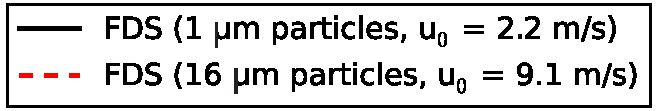
\includegraphics[width=3.5in]{Fig_Sippola_Aerosol_Deposition_Transverse_Legend.pdf}
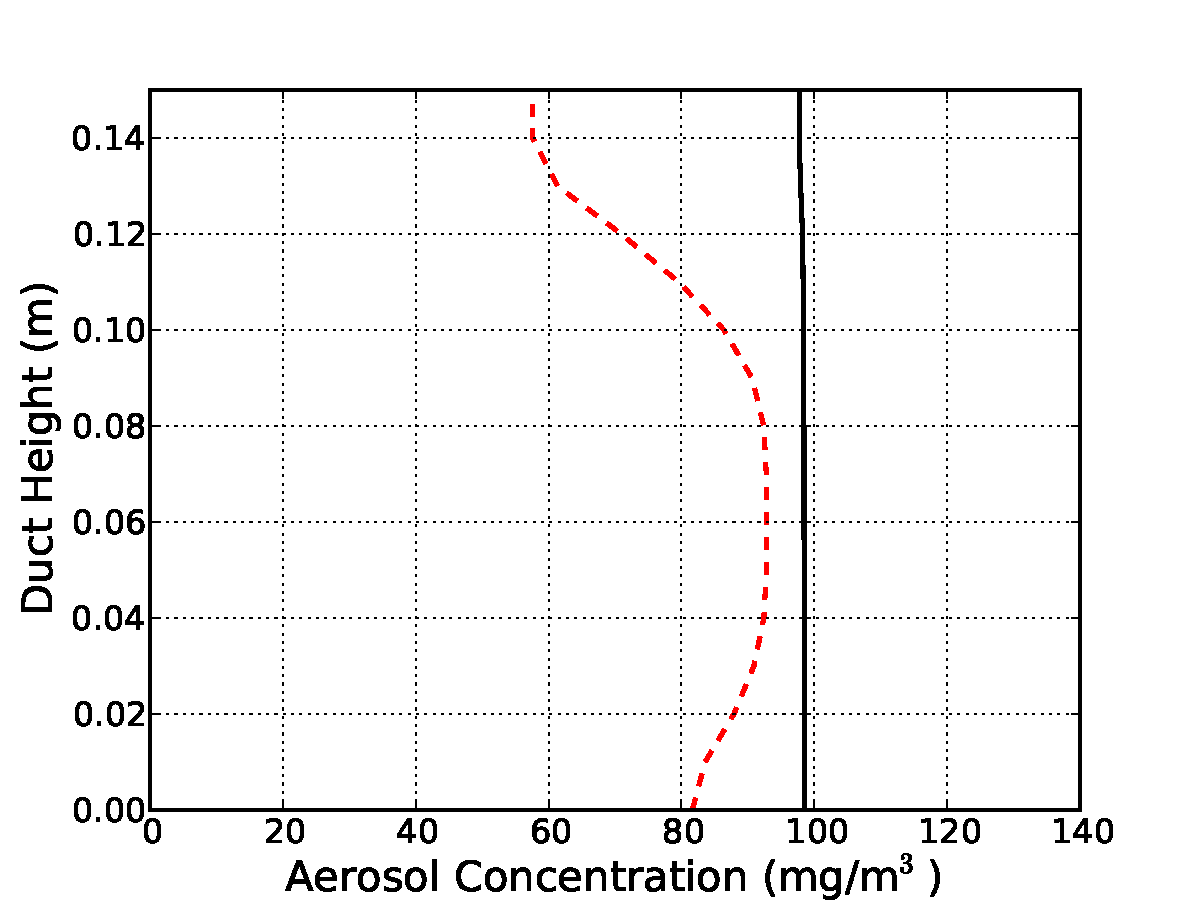
\includegraphics[width=5.0in]{Fig_Sippola_Aerosol_Deposition_Transverse_Concentration.pdf}
\caption[Vertical aerosol concentration profile, Sippola Aerosol Deposition]
{Vertical aerosol concentration profile 0.75~m downstream in the 1.5~m instrumented section of the duct for Test~1, 1~$\mu$m, 2.2~m/s case (solid line) and Test~16, 16~$\mu$m, 9.1~m/s case (dashed line).}
\label{fig:Sippola_Transverse_Concentration}
\end{figure}

\section{Conclusions}
\label{sec:Conclusions}

As a first approach of quantifying aerosol deposition predictions under non-reacting flow conditions, this study identified important parameters related to aerosol deposition under various flow conditions and compared predicted aerosol deposition quantities to experimentally measured data. To compare the predicted results to experimentally measured data, 16 tests conducted by Sippola~\cite{Sippola:1} were used in which ceiling, wall, and floor aerosol deposition velocities for various sizes of monodisperse fluorescent particles and various air velocities in a ventilation duct were measured. The experiments were numerically simulated, and the measured and predicted aerosol deposition velocities were compared and found to be underpredicted by 45~\%. Additional predicted quantities are presented such as the velocity profiles and aerosol concentrations in the duct as well as the aerosol concentration gradient along the duct.

In general, for all of the cases that were considered, the measurements and predictions indicate that, as the duct velocity and particle size increase, the deposition velocity also increases. The effect of increased particle sizes on the aerosol deposition velocities was the greatest at the floor, and the effect of increased duct velocity on the aerosol deposition velocities was the greatest at the wall and ceiling. The floor aerosol deposition velocities were the least sensitive to an increase in the duct velocity because gravitational settling was more dominant than turbulent deposition at the floor.

Sippola reported a 10~\% relative experimental uncertainty in the measured aerosol deposition velocities~\cite{Sippola:2002}. The model generally underpredicted the measured aerosol deposition velocity by 45~\%, on average. The results were mostly biased by errors in relatively small aerosol deposition velocities (on the order of $1 \times 10^{-5}$~m/s) for small particle sizes (3~$\mu$m and 5~$\mu$m) at the lowest air velocities. However, it was demonstrated that the effect of this error in the overall deposited soot mass would not be significant.

For all of the particle sizes and duct velocities that were considered, the results represent our best current ability to predict aerosol deposition velocities for the Sippola aerosol deposition experiments using FDS. Some limitations of this work are that the soot is currently represented in the model with a single (mean) particle size, and soot agglomeration is not currently considered. Additionally, because the experiments considered in this study were conducted under isothermal conditions, there was not an evaluation of the role of thermophoretic deposition in the total amount of deposited aerosol mass. Future work includes conducting validation studies for aerosol deposition in cases with soot generated from well-characterized fires and implementing a simple soot agglomeration mechanism to account for soot particles that can grow over time, which can also impact the rate of soot deposition to surfaces. Additionally, the ability to define, track, and evolve aerosol size distributions will likely improve the accuracy of the aerosol transport predictions. As these improved soot transport, deposition, and agglomeration mechanisms are implemented in the model, we can expect that the total amount of aerosol and soot deposition as well as the gas phase aerosol and soot concentrations will be more accurate. Additional verification and validation work on the soot and aerosol deposition routines in FDS can be found in the FDS Verification Guide~\cite{FDS_Verification_Guide}, FDS Validation Guide~\cite{FDS_Validation_Guide}, and Overholt~\cite{Overholt:Dissertation}.

\clearpage

% TEMPLATE INFORMATION

% \section{Introduction}
% \label{intro}
% Your text comes here. Separate text sections with
% \section{Section title}
% \label{sec:1}
% Text with citations \cite{RefB} and \cite{RefJ}.
% \subsection{Subsection title}
% \label{sec:2}
% as required. Don't forget to give each section
% and subsection a unique label (see Sect.~\ref{sec:1}).
% \paragraph{Paragraph headings} Use paragraph headings as needed.
% \begin{equation}
% a^2+b^2=c^2
% \end{equation}

% % For one-column wide figures use
% \begin{figure}
% % Use the relevant command to insert your figure file.
% % For example, with the graphicx package use
%   \includegraphics{example.eps}
% % figure caption is below the figure
% \caption{Please write your figure caption here}
% \label{fig:1}       % Give a unique label
% \end{figure}
% %
% % For two-column wide figures use
% \begin{figure*}
% % Use the relevant command to insert your figure file.
% % For example, with the graphicx package use
%   \includegraphics[width=0.75\textwidth]{example.eps}
% % figure caption is below the figure
% \caption{Please write your figure caption here}
% \label{fig:2}       % Give a unique label
% \end{figure*}
% %
% % For tables use
% \begin{table}
% % table caption is above the table
% \caption{Please write your table caption here}
% \label{tab:1}       % Give a unique label
% % For LaTeX tables use
% \begin{tabular}{lll}
% \hline\noalign{\smallskip}
% first & second & third  \\
% \noalign{\smallskip}\hline\noalign{\smallskip}
% number & number & number \\
% number & number & number \\
% \noalign{\smallskip}\hline
% \end{tabular}
% \end{table}

%\begin{acknowledgements}
%If you'd like to thank anyone, place your comments here
%and remove the percent signs.
%\end{acknowledgements}

% BibTeX users please use one of
% \bibliographystyle{spbasic}      % basic style, author-year citations
% \bibliographystyle{spmpsci}      % mathematics and physical sciences
% \bibliographystyle{spphys}       % APS-like style for physics
\bibliographystyle{unsrt}
\bibliography{references}   % name your BibTeX data base

% Non-BibTeX users please use
% \begin{thebibliography}{}
%
% and use \bibitem to create references. Consult the Instructions
% for authors for reference list style.
%
% \bibitem{RefJ}
% Format for Journal Reference
% Author, Article title, Journal, Volume, page numbers (year)
% Format for books
% \bibitem{RefB}
% Author, Book title, page numbers. Publisher, place (year)
% etc
% \end{thebibliography}

\end{document}
% end of file template.tex
